% !TeX spellcheck = en_US
\chapter{Git and GitHub}


    %------------------------------------------------------------------------------------------------------
    \section{Introduction}
    
Version Control Systems (VCS) are in charge of registering all the modifications made on a bunch of files, saving copies of the files, 
recording what changes have been made, at what time, by who, etc. 
The following actions can be carried out by a version control system such as Git: 

\begin{enumerate}
    \item Old versions of the project can be recovered in the future.
    \item The evolution on the project can be tracked.
    \item It is easier to collaborate on the same project with a group of people.
    \item Incompatible or simultaneous changes in the same files can be managed by conflict resolution tools.
\end{enumerate}

The VCS Git is one of the most popular choices but not the only one, it is created for tracking changes in computer files and making it ideal for software development (individual and among groups). 
Once it is installed in the computer any project can be managed by Git, that project is then called repository.
Since then, a \texttt{.git} hidden folder and some other files (i.e. the file \texttt{.gitignore}) appear in the repository.
In order to use it the command \texttt{git} is available on the command line, also, some integrated tools are common on IDEs like Visual Studio.

On the contrary, GitHub is a web-based hosting service made for Git where any registered user can publicly or privately post their repositories. 
With GitHub or similar remote services the code is stored and is accessible from around the world, multiple people can develop the same project at the same time
and it is fully integrated with Git.

This chapter explains how to install Git and GitHub tools on Visual Studio and summarizes the most basic commands in order to use Git properly in our projects. 




    %------------------------------------------------------------------------------------------------------
    \section{Installing...}
   
The main characters in the VCS explained in this chapter are the following, consider which of them can be useful for your situation.  

\begin{itemize}
    \item Git 
    \item GitHub account
    \item GitHub Extension for Visual Studio, GitHub Desktop or both
    \item GitHub Classroom account
\end{itemize}
   
First of all, in order to use all the tools mentioned here, get sure that you already have a GitHub account, whether it is personal or with your institutional email. If GitHub classroom is going to be used it is recommended the institutional email. 
    
To install Git an executable installer can be freely obtained from its main website: \underline{https://git-scm.com/}. Look for your operating system and download the installer, then install it in your computer by following the steps. Another option is to install Git from the Visual Studio installer; open and update it, go to Individual Components tab and find ``GIT for Windows'', select it and click on ``Modify''. Both ways install the tool for your computer, independently of using it with Visual Studio, a different IDE or the command prompt.

Once finished, by opening a command line you should be able to execute a git command, for example type: \texttt{git help git} on your command window, the Manual page should open in your browser. Now, git is available in your computer and it can be used in many different projects like \LaTeX documents, Visual Studio solutions (\texttt{.sln}), MATLAB projects, etc. 

In order to fully use GitHub integrated with all the projects mentioned before different options are available:

\begin{enumerate}
    \item If you are using Visual Studio install the GitHub extension in the IDE. Open EXTENSIONS and click on ``Manage Extensions'', open the tab ``Online'', look for the GitHub tool and install it. 
    \item If your IDE does not have a GitHub integrated tool you can also manage it with GitHub Desktop, an application that brings and extents the potential of GitHub independently of the IDE used or the project being developed. 
\end{enumerate}


%Crear Git repository o clonar uno existente
%Ya sea local o remoto
%Flujo de trabajo en ambas herramientas
%gitignore es LO PRIMERO QUE HAY QUE CREAR y readme creo que tambien



\newpage 
\section{Workflow in Git and GitHub}
    
    
    
\begin{figure}[h]
    \centering
    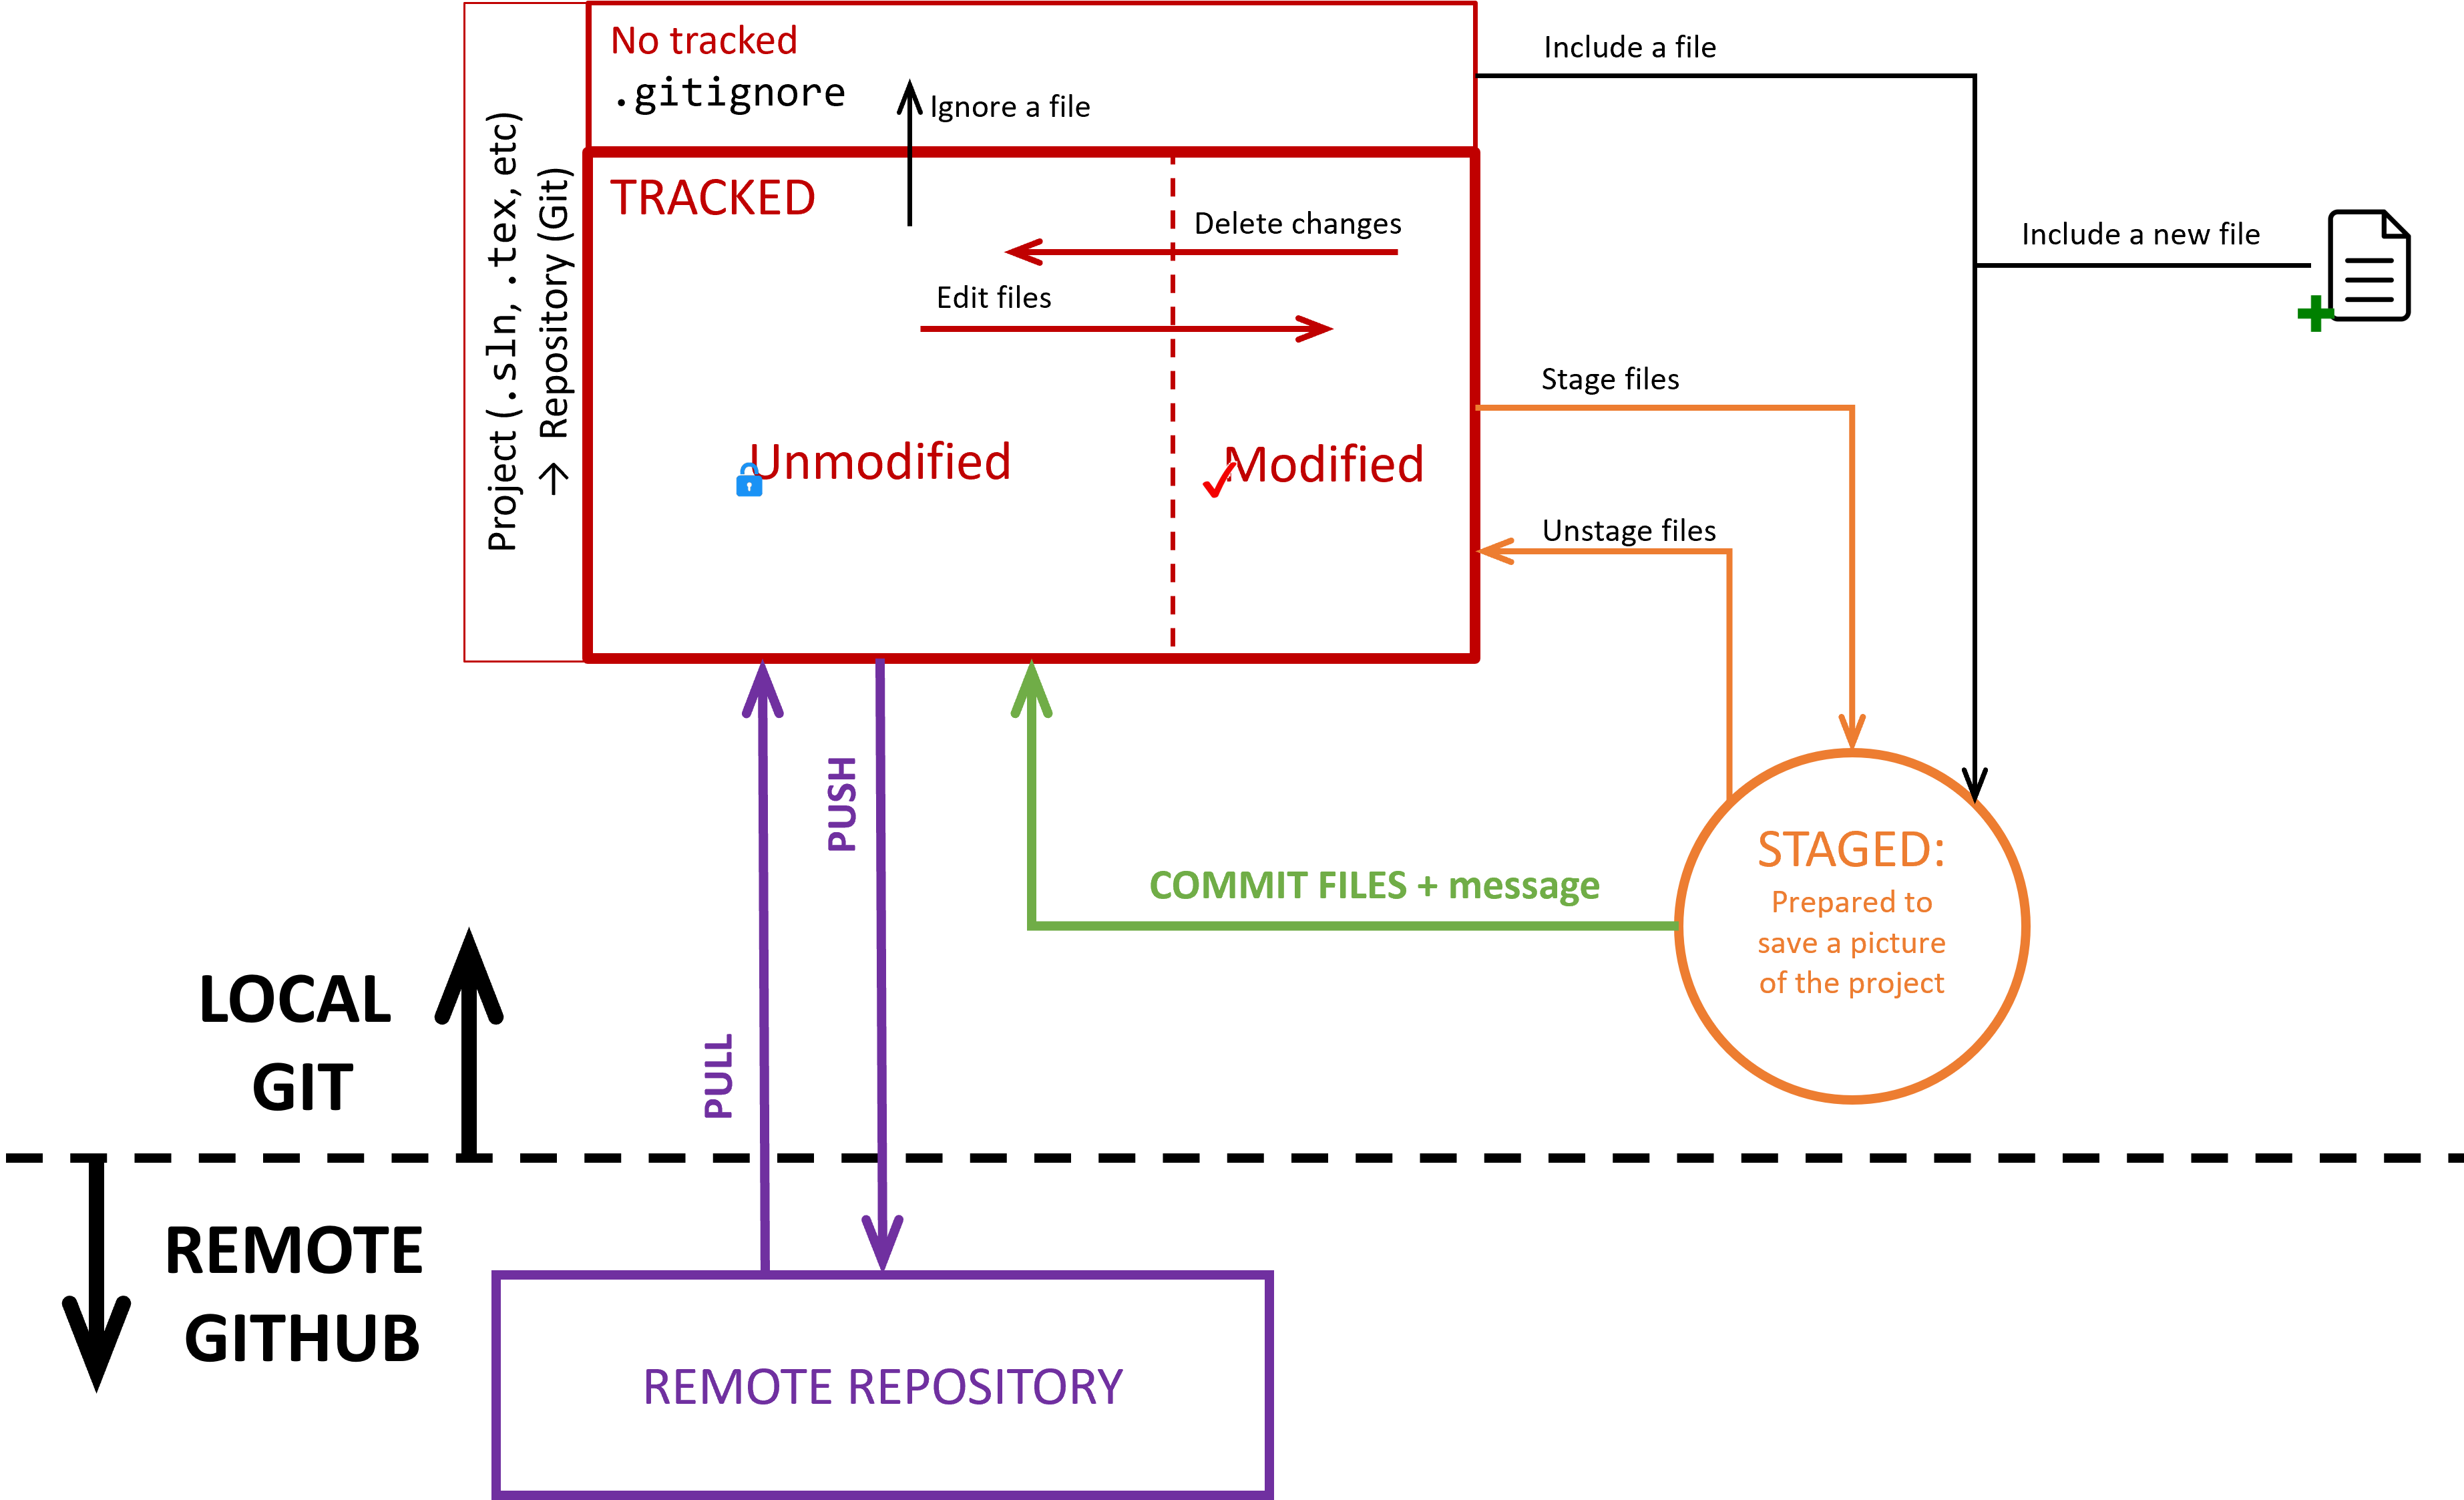
\includegraphics[width = 1.2\textwidth]{Figures/GHStates.png}
    \caption{Git + GitHub workflow main states.}
    \label{fig:GitStates}
\end{figure} 
  
\section{Create GitHUB repository from local project}



















    
%    \section{Create a Git repository of a solution}
%
%To add a Git repository to the solution proceed with the following steps:
%
%\begin{enumerate}
%    \item Open your version of Visual Studio.
%    \item Open the solution.
%    \item In the solution explorer, right click on the name of your solution and select \textit{Add Solution to Source Control...} (Figure \ref{fig:Git0}).
%    \item Click on \textit{View/Team Explorer} and check that the repository has been created (Figure \ref{fig:Git1}).
%\end{enumerate}
%
%\begin{figure}[h]
%    \centering
%    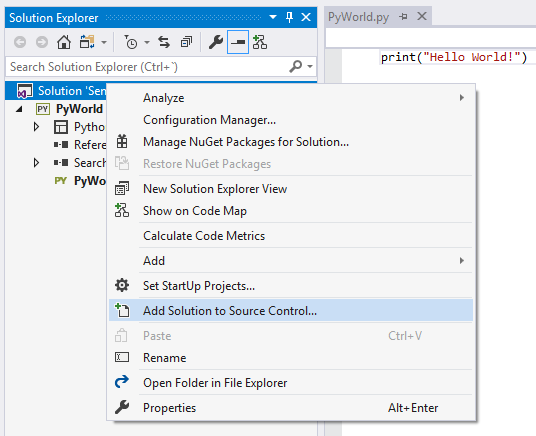
\includegraphics[width=0.7 \textwidth]{Figures/G0V1.png}
%    \caption{Adding Version Control to an existing Visual Studio solution.}
%    \label{fig:Git0}
%\end{figure}
%
%\begin{figure}[h]
%    \centering
%    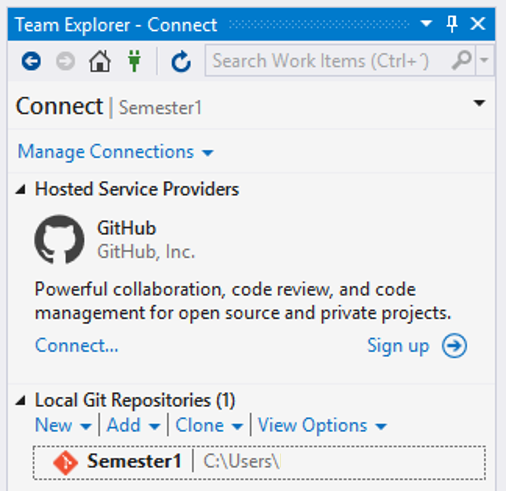
\includegraphics[width=0.5 \textwidth]{Figures/G1V2.png}
%    \caption{\textit{Team Viewer} tab. The solutions with Git repositories are shown in the \textit{Local GIT repositories} menu.}
%    \label{fig:Git1}
%\end{figure}
%
%%\begin{figure}[h]
%%\centering
%%\caption{New Git repo.}
%%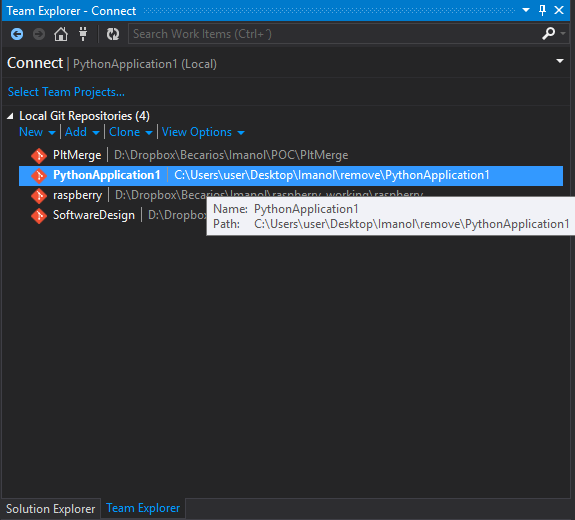
\includegraphics[width=0.85 \textwidth]{Figures/git2.PNG}
%%\label{fig:Git2}
%%\end{figure}
%
%    \section{Save changes on a Git repository}
%
%While developing a software project a large number of files are modified, renamed and deleted. Periodically we want to save all the changes performed in a work session by updating the repository. In order to do that, follow these steps:
%
%\begin{enumerate}
%    \item Open an existing Visual Studio solution with a Git repository.
%    \item Click on \textit{View/Team Explorer} or on \textit{Team Viewer} tab.
%    \item Click on the \textit{Home} icon (
\includegraphics[height=11pt]{./Figures/Home.png}).
%    \item Click on \textit{Changes}.
%    \item Write a short comment on the text area (Figure \ref{fig:GitCommit0}).
%    \item Click on \textbf{confirm all}.
%\end{enumerate}
%
%\begin{figure}[h]
%    \centering
%    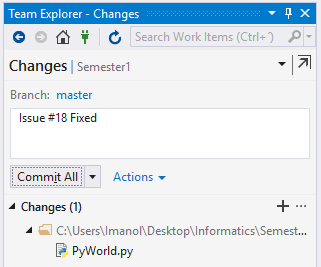
\includegraphics[width=0.5 \textwidth]{Figures/GCV2.png}
%    \caption{\textit{Changes} section of the \textit{Team Viewer} tab. In this case the script \textit{PyWorld.py} has changed since the last version updated and it is going to be saved again.}
%    \label{fig:GitCommit0}
%\end{figure}
%
%
%
%
%    \section{Configure GitHub}
%
%If we have already installed the GitHub extension we can configure our account. The following steps describe how to upload our projects to the web with the GitHub account:
%
%\begin{enumerate}
%	\item Open Visual Studio.
%	\item Open an existing solution with a Git repository.
%	\item On \textit{View/Team Explorer} and click on the \textit{Home} icon.
%	\item Click on \textit{Sync}.
%	\item In the \textit{Publish to GitHub} section, click on \textit{Sign in} in order to log in with your account (Figure \ref{fig:GitHub0}).
%	\item Push the repository to GitHub (Figure \ref{fig:GitHub2}).
%\end{enumerate}
%
%\begin{figure}[h]
%	\centering
%	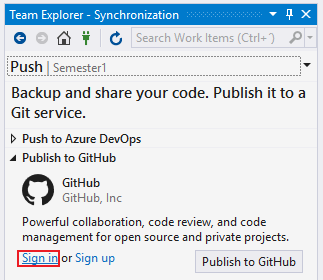
\includegraphics[width=0.5\textwidth]{Figures/GH0V3.png}
%	\caption{\textit{Sync} tab of the Team Viewer. Git repositories can be published on remote servers such as \textit{Team Services} or \textit{GitHub}.}
%	\label{fig:GitHub0}
%\end{figure}
%
%%\begin{figure}[h]
%%	\centering
%%	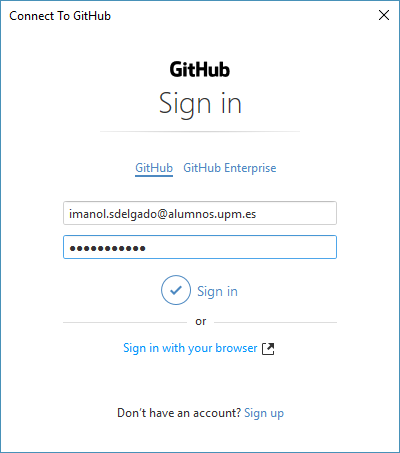
\includegraphics[width=0.4\textwidth]{Figures/GH1.png}
%%	\caption{GitHub Sign in window.}
%%	\label{fig:GitHub1}
%%\end{figure}
%
%\begin{figure}[h]
%	\centering
%	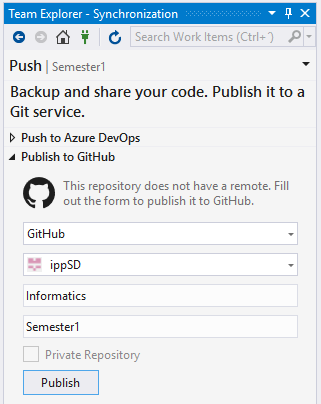
\includegraphics[width=0.5\textwidth]{Figures/GH2V3.png}
%	\caption{\textit{Sync} tab in the Team Viewer. If we have a \textit{GitHub} account we can publish our Git repositories.}
%	\label{fig:GitHub2}
%\end{figure}
%
%    \section{Import projects from GitHub}
%
%Visual Studio can create solutions from the source code of remote repositories obtained from GitHub thanks to the extension installed in the previous sections. In order to import a repository follow this:
%
%\begin{enumerate}
%	\item Go to \textit{View/Team Explorer} as usual.
%	\item Click on the \textit{Manage Connections} icon (
\includegraphics[height=11pt]{./Figures/Connect.png}).
%	\item In the \textit{GitHub} section select \textit{clone}.
%	\item Select a \textit{Repository name} (Figure \ref{fig:GitHubClone1}).
%	\item Select a \textit{path} for saving the repository.
%	\item Click on \textit{Clone}.
%	\item Go to the \textit{Team Viewer} tab and click on \textit{Manage Connections} icon once again (Figure \ref{fig:GitHubClone2}).
%	\item Double click on the downloaded \textit{Repository name}.
%	\item If there is no solution on the \textit{Solutions} section, select \textit{New...} in order to create it.
%	\item Create a solution for the repository according to the programming language of the source code.
%\end{enumerate}
%
%\begin{figure}[H]
%	\centering
%	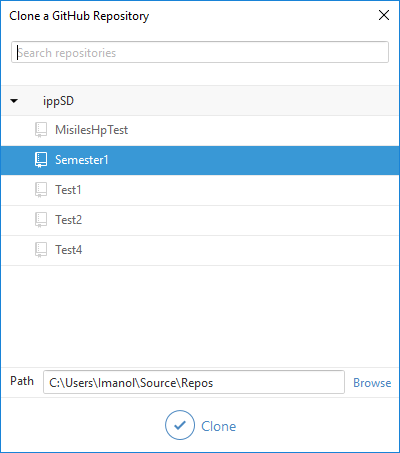
\includegraphics[width=0.5\textwidth]{Figures/GHC1.png}
%	\caption{Available Git repositories list on a GitHub account that can be cloned by Visual Studio.}
%	\label{fig:GitHubClone1}
%\end{figure}
%
%\begin{figure}[H]
%	\centering
%	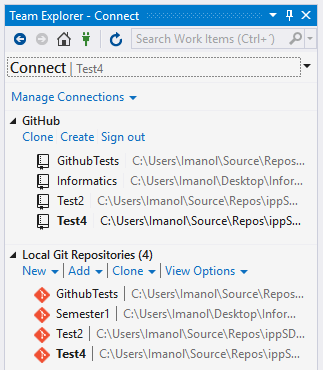
\includegraphics[width= 0.5\textwidth]{Figures/GHC3V3.png}
%	\caption{Available local Git repositories.}
%	\label{fig:GitHubClone2}
%\end{figure}
%
%    \section{Download repository updates from GitHub}
%
%While working as a team, it is possible that two or more people make changes on the remote repository at the same moment. These changes must be \textbf{pulled} from GitHub in order to have an updated version of the code and make sure that all members work on the same source files. In order to check the updates, follow the next steps:
%
%\begin{enumerate}
%	\item Go to \textit{View/Team Explorer} and click on the \textit{Home} icon.
%	\item Click on \textit{Sync}.
%	\item Select \textit{Recover} in order to getting the changes from the remote repository.
%	\item Click on \textit{Extract} for applying those changes.
%\end{enumerate}
%
%    \section{Upload local changes to GitHub}
%
%Once our project is ready, it has to be \textbf{pushed} to the remote repository so that every team member has access to the last updates. This can be made by following these steps:
%
%\begin{enumerate}
%	\item Commit changes of the current project.
%	\item Go to \textit{View/Team Explorer} (or the \textit{Team Viewer} tab) and click on the \textit{Home} icon.
%	\item Click on \textit{Sync}.
%	\item Click on \textit{sync} for automatically synchronize all commits.
%\end{enumerate}
%
%    \section{Avoid uploading specific files to the repository}
%
%When saving changes to the Git repository, all files generated by the project such as compiled, temporary or output files are included. We might not want all of them to be uploaded, just source code and documentation for example. Git includes a configuration file, \textbf{gitignore}, where the files and folders to be skipped are recorded. In order to edit this file follow the next steps:
%
%\begin{enumerate}
%	\item Open a Git configured Visual Studio solution.
%	\item Go to \textit{Team Viewer} tab and click on the \textit{Home} icon.
%	\item Click on the \textit{Settings} button and select \textit{Repository Settings}.
%	\item Unfold the \textit{Ignore \& Attributes Files} menu and click on the \textit{Edit} link next to \textit{Ignore File} (Figure \ref{fig:GitIgnore0}).
%	\item Edit the \textit{gitignore} file.
%\end{enumerate}
%
%\begin{figure}[h]
%	\centering
%	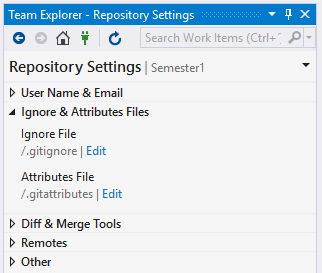
\includegraphics[width= 0.7\textwidth]{Figures/GIG0.png}
%	\caption{Menu for accessing the Gitignore file.}
%	\label{fig:GitIgnore0}
%\end{figure}
%
%\textit{gitignore} uses \textit{Regex} (Regular Expressions) syntax for selecting files. Figure \ref{fig:GitIgnore1} shows an example with the most common expressions:
%
%\begin{itemize}
%	\item All lines: text placed after the hash symbol (\#) are comments with no real effect.
%	\item Line 266: asterisk (*) matches any text. In this case, files ending with \textit{pyc} extensions are omitted.
%	\item Line 268: double asterisk (**) matches any folder. In this case, the \textit{\_\_pycache\_\_} folder is omitted on all subdirectories of the repository.
%	\item Lines 273, 274: Regex syntax can be used multiple times on the same line. In these cases, folders containing \textit{Advisor} or \textit{OLD} are omitted from all subdirectories of the repository.
%	\item Line 272: Characters inside square brackets ([...]) are used for text combinations. In these cases, \textit{Debug}, \textit{debug}, \textit{DebugPublic}, \textit{debugPublic} folders are omitted.
%\end{itemize}
%
%\begin{figure}[h]
%	\centering
%	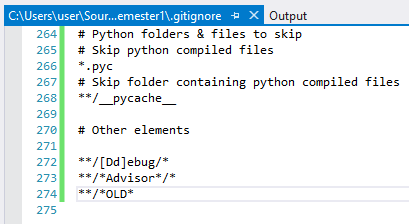
\includegraphics[width= 0.8\textwidth]{Figures/GIG1.png}
%	\caption{Gitignore example.}
%	\label{fig:GitIgnore1}
%\end{figure}
%
%    \section{Git and GitHub FAQ}
%
%\begin{itemize}
%    
%    %%%%%%%%%%%%%%%%%%%%%%%%%%%%%%%%%%%%%%%%%%%%%%%%%%%%%%%%%%%%%%%%%%%%%%%%%%%%%%%%%%%%%%%%%%%%%%%
%	\item \textbf{I can not save changes on GitHub: Updates were rejected because the remote contains work that you do not have locally}.
%	
%	This occurs because there were changes on the remote repository that you did not updated. Since you have modified outdated files, now there are conflicts on the files and it has to be solved manually. You have to download them first and then upload the new code:
%	
%	\begin{enumerate}  
%		\item Go to \textit{Team Viewer} tab and click on the \textit{Home} icon.
%		\item Click on \textit{Sync}.
%		\item Click on \textit{Recover}. The new changes should appear.
%		\item Click on \textit{sync}.
%		\item There might be errors on merging (Figure \ref{fig:GitHubErr1}).
%		\item Click on \textit{Conflicts}.
%		\item Select a \textit{conflict file}.
%		\item There are several ways of solving conflicts (Figure \ref{fig:GitHubErr2}):
%		\begin{enumerate}
%			\item \textit{Take remote} file and discard local changes.
%			\item \textit{Keep local changes} and override remote file.
%			\item \textit{Merge by combination} both files and select code to be kept and discard.
%		\end{enumerate}
%    	\item Sync again.
%        %\begin{figure}[h]
%        %	\centering
%        %	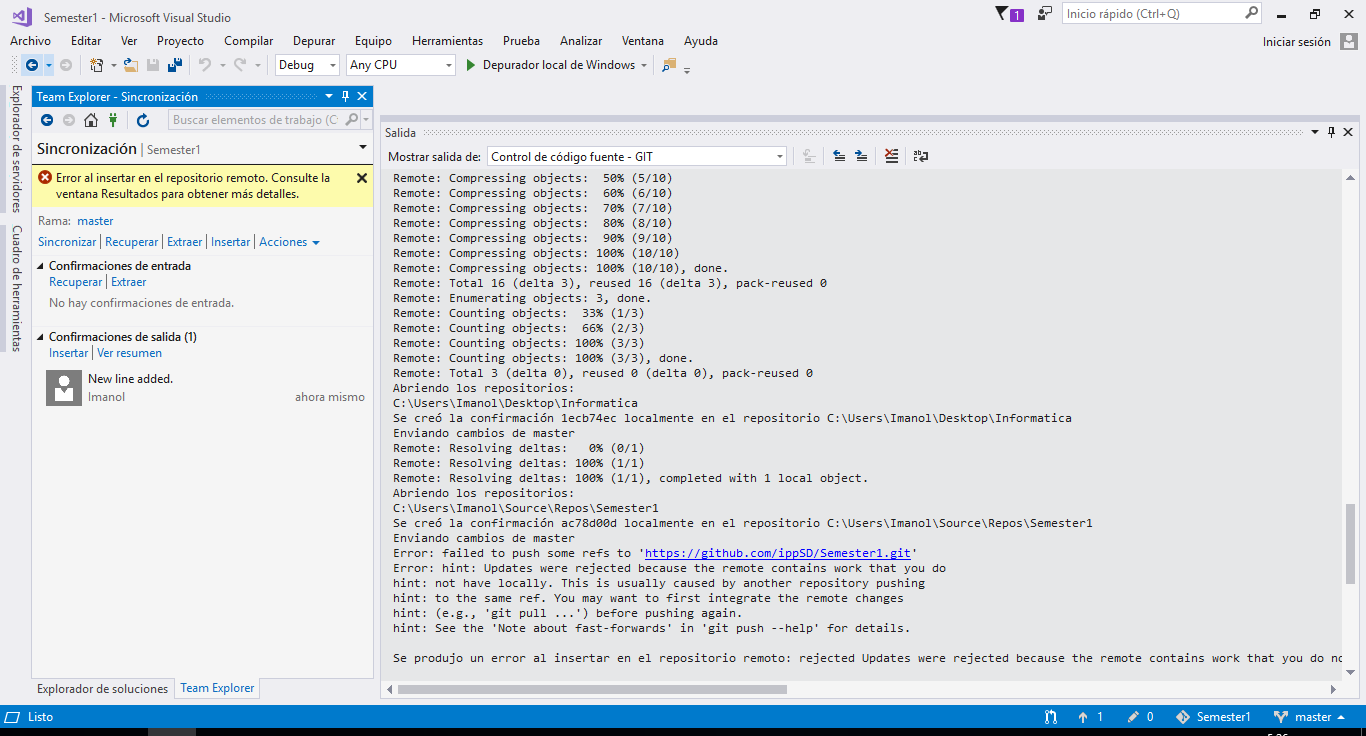
\includegraphics[width=\textwidth]{Figures/GHERR0.png}
%        %	\caption{Common Git error o}
%        %	\label{fig:GitHubErr0}
%        %\end{figure}
%        
%        \begin{figure}[h]
%        	\centering
%        	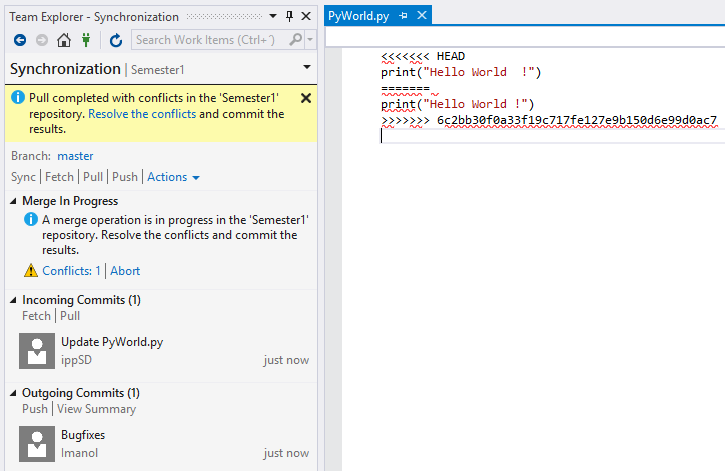
\includegraphics[width=\textwidth]{Figures/GHERR1V1.png}
%        	\caption{Solving conflicts with local and remote repositories, step 1.}
%        	\label{fig:GitHubErr1}
%        \end{figure}
%        
%        \begin{figure}[h]
%        	\centering
%        	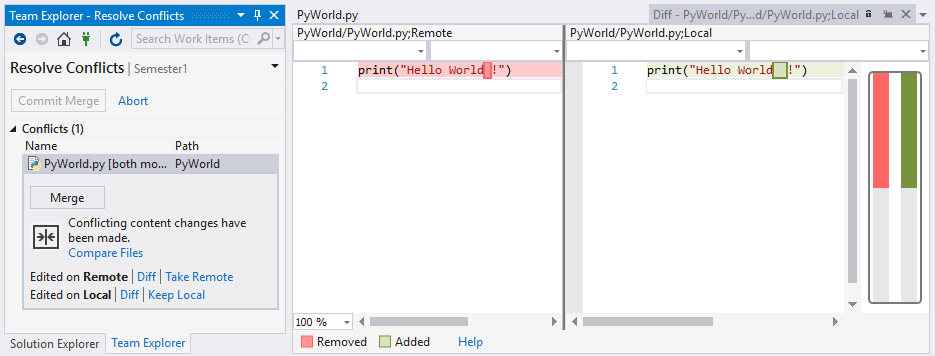
\includegraphics[width=\textwidth]{Figures/GHERR2V1.png}
%        	\caption{Solving conflicts with local and remote repositories, step 2.}
%        	\label{fig:GitHubErr2}
%        \end{figure}	
%	\end{enumerate}
%	
%    %%%%%%%%%%%%%%%%%%%%%%%%%%%%%%%%%%%%%%%%%%%%%%%%%%%%%%%%%%%%%%%%%%%%%%%%%%%%%%%%%%%%%%%%%%%%%%%
%	\item \textbf{How can I unbind a project from GitHub?}
%	
%	A local Git repository can be unlinked from the remote repository on the configuration settings:
%	
%	\begin{itemize}
%		\item Go to \textit{Team Viewer} tab as usual and click on the \textit{Home} icon.
%		\item Click on \textit{Configuration}.
%		\item Click on \textit{Repository Configuration}.
%		\item In the \textit{remote} section, click on \textit{remove}.
%	\end{itemize}
%
%    %%%%%%%%%%%%%%%%%%%%%%%%%%%%%%%%%%%%%%%%%%%%%%%%%%%%%%%%%%%%%%%%%%%%%%%%%%%%%%%%%%%%%%%%%%%%%%%
%	\item \textbf{I changed the \textit{gitignore} file but the omitted files are still being uploaded}
%	
%	This occurs when the files/folders to be omitted where first saved in the repository and then included on the \textit{gitignore} file. In order to fix this issue, a quick workaround is made:
%	
%	\begin{enumerate}
%		\item Save changes to the git repository. This commit will serve as a backup.
%		\item Move all the files/folders you want to omit out of the solution directory.
%		\item Save the new changes to the git repository. Displaced files will be removed from the repository.
%		\item Restore the moved files/folders on their original directories.
%		\item Save the new changes to the git repository. Due to omitted files being removed and \textit{gitignore} blocking them these files will not appear again.
%	\end{enumerate}
%
%
%    %%%%%%%%%%%%%%%%%%%%%%%%%%%%%%%%%%%%%%%%%%%%%%%%%%%%%%%%%%%%%%%%%%%%%%%%%%%%%%%%%%%%%%%%%%%%%%%
%	\item \textbf{How can I upload files to GitHub without Visual Studio?}
%		
%	Source code, graphics, documentation, etc. can be uploaded to GitHub without using the \textit{Team Viewer} window by using either \textbf{Git Command Line Tools} or the \textbf{GitHub Web Page}. Since command line tools require additional software, only the web approach will be explained. 
%		
%%		\subsubsection*{\textbf{Git Command Line Tools}}
%%		
%%		\begin{enumerate}
%%			\item Right click on \textit{??}.
%%			\item Place files and folders on said folder.
%%			\item Add and commit new files to the repository:
%%\begin{lstlisting}
%%$ git add *
%%$ git commit -m "COMMIT MESSAGE"\end{lstlisting}
%%			\item Add your remote repository location, \textit{REPOSITORY-URL}. The remote address will be aliased as \textit{origin}.
%%\begin{lstlisting}
%%$ git remote add origin "REPOSITORY-URL" \end{lstlisting}
%%			\item Push changes to GitHub:
%%\begin{lstlisting}{bash}
%%$ git push -u origin master\end{lstlisting}
%%		\end{enumerate}
%		
%    %\subsubsection*{\textbf{GitHub Web Page}}
%    
%    Files and folder can be easily saved by dropping them onto the web browser.
%    
%    \begin{enumerate}
%    	\item Log in \textit{https://github.com} with your credentials.
%    	\item Open the GitHub repository page where files must be stored.
%    	\item On the \textit{Code} tab, click on \textit{Upload Files} button.
%    	\item Drag the files and folders onto the browser.
%    	\item \textit{Commit} changes before closing the web page. 	
%    \end{enumerate}	
%\end{itemize}
%
%\begin{figure}[h]
%	\centering
%	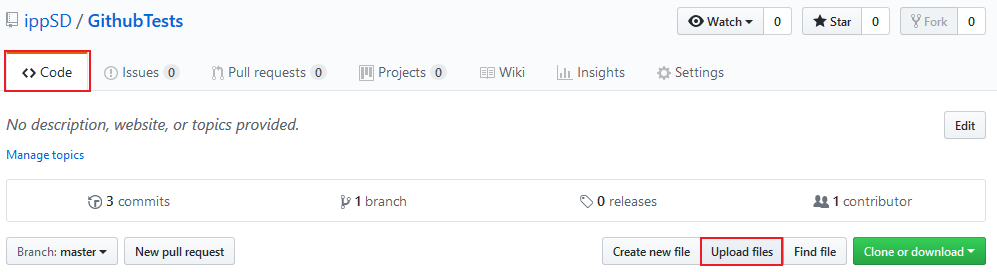
\includegraphics[width=\textwidth]{Figures/GUP0.png}
%	\caption{How to upload files to GitHub manually (first step).}
%	\label{fig:GitHubUpload0}
%\end{figure}
%
%\begin{figure}[h]
%	\centering
%	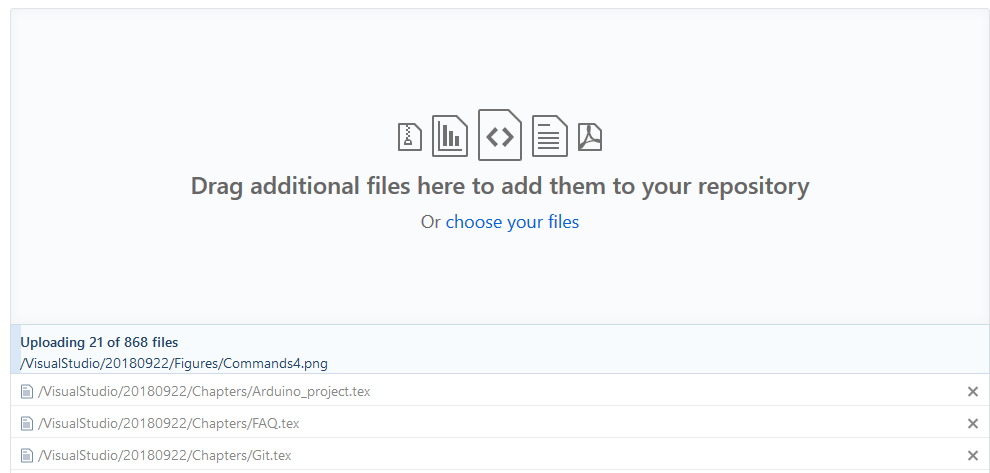
\includegraphics[width= \textwidth]{Figures/GUP1.png}
%	\caption{How to upload files to GitHub manually (second step).}
%	\label{fig:GitHubUpload1}
%\end{figure}
%
%\begin{figure}[h]
%	\centering
%	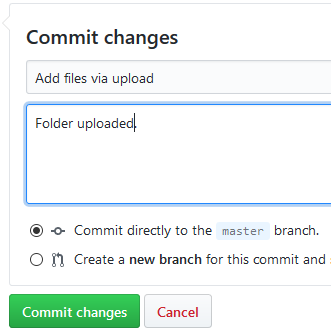
\includegraphics[width=0.5 \textwidth]{Figures/GUP2.png}
%	\caption{How to upload files to GitHub manually (third step).}
%	\label{fig:GitHubUpload2}
%\end{figure}



























%\clearpage
%\section{Visual Studio Git commands}
%
%When a project is selected on \textbf{Team Explorer} panel there are several 
%options available by expanding the top horizontal bar:
%
%\begin{itemize}
%\item \textbf{Changes}: includes the project saving commands.
%\item \textbf{Branches}: manages branches of the repository.
%\item \textbf{Unsynced Commits}: allows remote operations.
%\item \textbf{Settings}: Git settings.
%\end{itemize}
%
%\subsection{Bind Visual Studio to a person}
%
%On team working the username and email address is compulsory so it has to be 
%changed on Git Settings.
%
%\begin{enumerate}
%\item Set username and email:
%On \textbf{Team Explorer} panel and on your Git repository, Select on the top 
%horizontal bar \textbf{``Settings{$\rightarrow$}Git Settings''}. Add/change 
%\textbf{User Name} and \textbf{Email Address}, then press \textbf{Update}
%\end{enumerate}
%
%\subsection{Commit your code}
%
%\begin{enumerate}
%\item On \textbf{``Team Explorer''} panel, select your Git repository and go to 
%\textbf{``Changes''}.
%
%\item If you want to hide a file/folder from your repository (``OLD'' folders, 
%``*.bak'' files, etc.), on the \textbf{``Included Changes''} tree select your 
%folder/file and select \textbf{``Exclude''}.
%
%\item If you want to add a new version of an excluded folder/file, right click 
%and \textbf{``Include''} on the \textbf{``Excluded Changes''} tree.
%
%\item Set a \textbf{``commit message''} and hit the \textbf{``commit''} button.
%\ref{fig:Git3}
%
%
%\begin{figure}[h]
%\centering
%\caption{Git ``Changes'' option.}
%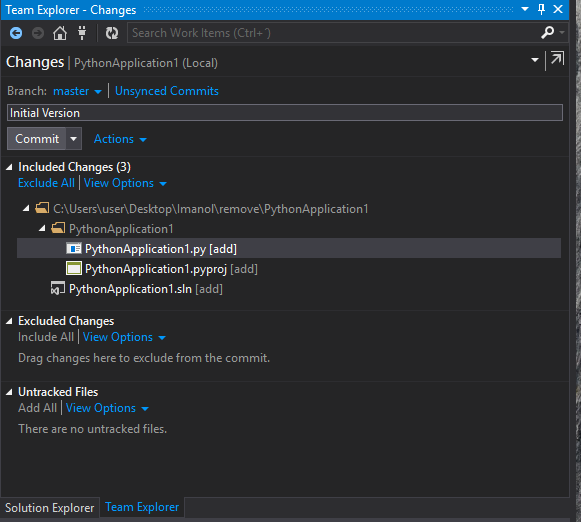
\includegraphics[scale=0.6]{Figures/git3.PNG}
%\label{fig:Git3}
%\end{figure}
%
%\end{enumerate}






%%%%%%%%%%%%%%%%%%%%%%%%%%%%%%%%%%%%%    OLD    %%%%%%%%%%%%%%%%%%%%%%%%%%%%%%%%%%%%%%%%%%%

% According to Visual Studio Documentation, VCS are defined in the following way:
%
%\begin{center}
%    \begin{minipage}{0.7\linewidth}
%        \vspace{5pt}        %margen superior de minipage
%        {\small
%            ``Version control systems help you track changes to code over time. 
%            As you make changes, the version control system takes a snapshot of 
%            your files. The version control system saves that snapshot 
%            permanently so you can recall it later if you need it...''
%        }
%        \begin{flushright}
%            (\url{https://docs.microsoft.com/en-us/visualstudio/version-control/?view=vs-2017})
%        \end{flushright}
%        \vspace{5pt}%margen inferior de la minipage
%    \end{minipage}
%\end{center}


%natively, Git included. For 
%an easy experience Visual Studio offers a simple GUI so that only a little 
%concepts are required.
%
%Git with Visual Studio can clone a remote project from GitHub, GitLab or even a 
%custom server in order to work as a team.

%\section{Git most important commands}
%
%This section explains the basic Git commands and provides a better 
%understanding of how to work on Git.
%
%\subsection*{Commands for creating a project}
%Initialization commands:
%
%\begin{itemize}
%\item \textbf{init}: create an empty Git repository.
%\item \textbf{clone}: download a Git repository from an URL or a local 
%directory.
%\end{itemize}
%
%\subsection*{Commands for saving a project}
%
%Once on a working Git repository, new created and modified files must be added 
%to a queue so that they are added to the repository when necessary. These are 
%the basic commands:
%
%\begin{itemize}
%\item \textbf{add}: add files and folders to your repository's changes queue. 
%Some will appear as new, others as modified and some even as renamed.
%\item \textbf{commit}: uploads the changes queue to the repository. Now the 
%changes have been submitted and the changes queue is empty.
%\end{itemize}
%
%\subsection*{Commands for making branches}
%
%Branches allow the user to separate ways from a common origin, which means that 
%changes on a branch will not affect to others. It is useful for having a 
%working and compiling project (e.j. \textit{master}) and a testing branch (e.j. 
%\textit{dev}) so that when the testing works it can be uploaded to the main 
%project.
%\begin{itemize}
%\item \textbf{branch}: create a new branch from another one, being 
%\textit{master} as the default branch, or destroy an existing one. It creates a 
%new branch but it does not use it, so use the \textit{checkout} command before 
%editing anything else.
%\item \textbf{checkout}: change the working branch.
%\item \textbf{merge}: combines branches.
%\end{itemize}
%
%\subsection*{Commands for remote repositories}
%
%\begin{itemize}
%\item \textbf{pull}: get a commit, branch, etc. from remote.
%\item \textbf{push}: upload commit, branch, etc. to remote.
%\end{itemize}






%    \FloatBarrier
%    \section{Installing GitHub Extension}
%
%Visual Studio includes a GitHub extension for saving Git repositories on-line on your account. In order to install the extension follow these steps:
%
%\begin{enumerate}
%	\item Click on \textit{Tools/Extensions and Updates...}
%	\item Click on the tab ``Online'' on the left part of the window and then search for ``GitHub Extension for Visual Studio'' (you can use the Search engine).
%    \item Download it (Figure \ref{fig:GitHubTest0}).
%	\item Close all Visual Studio windows and follow the instructions of the \textit{GitHub extension installer} program.
%    \item The process will finish automatically after clicking on \textit{Modify} in one of the steps.
%\end{enumerate}
%
%\begin{figure}[h]
%	\centering
%	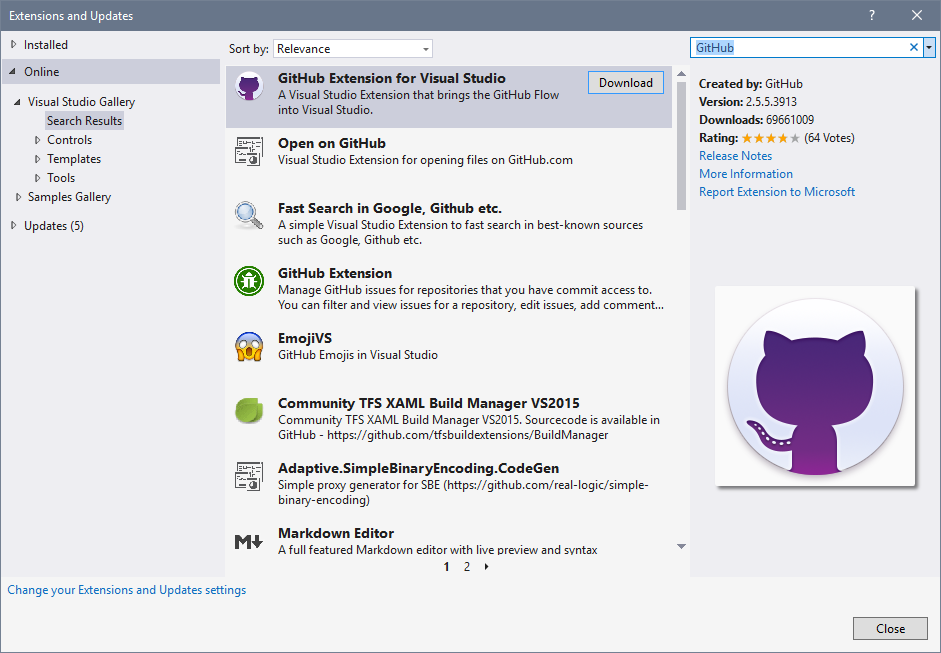
\includegraphics[width=\textwidth]{Figures/GH-1.png}
%	\caption{\textit{Extensions and updates} window of VS where the GitHub extension can be installed, updated or removed.}
%	\label{fig:GitHubTest0}
%\end{figure}\section{Create GitHUB repository from local project}